\documentclass{article}

\usepackage{arxiv}

\usepackage[utf8]{inputenc} % allow utf-8 input
\usepackage[T1]{fontenc}    % use 8-bit T1 fonts
\usepackage{lmodern}        % https://github.com/rstudio/rticles/issues/343
\usepackage{hyperref}       % hyperlinks
\usepackage{url}            % simple URL typesetting
\usepackage{booktabs}       % professional-quality tables
\usepackage{amsfonts}       % blackboard math symbols
\usepackage{nicefrac}       % compact symbols for 1/2, etc.
\usepackage{microtype}      % microtypography
\usepackage{graphicx}
\usepackage{amsmath}
\usepackage{float}
\usepackage{enumitem}
\usepackage{subcaption}

\title{Replication of Crypto Factor Analysis}

\author{
    \small
    \begin{minipage}[t]{0.24\textwidth}
        \centering
        Daniel Liang \\
        Master of Science in Finance \\
        University of Illinois \\
        \texttt{\href{mailto:yuanhui5@illinois.edu}{\nolinkurl{yuanhui5@illinois.edu}}}
    \end{minipage}
    \hfill
    \begin{minipage}[t]{0.24\textwidth}
        \centering
        Zixuan Feng \\
        Master of Science in Finance \\
        University of Illinois \\
        \texttt{\href{mailto:zf20@illinois.edu}{\nolinkurl{zf20@illinois.edu}}}
    \end{minipage}
    \hfill
    \begin{minipage}[t]{0.24\textwidth}
        \centering
        Xiyu Cai \\
        Master of Science in Finance \\
        University of Illinois \\
        \texttt{\href{mailto:xiyucai2@illinois.edu}{\nolinkurl{xiyucai2@illinois.edu}}}
    \end{minipage}
    \hfill
    \begin{minipage}[t]{0.24\textwidth}
        \centering
        Weihua Zhang \\
        Master of Science in Finance \\
        University of Illinois \\
        \texttt{\href{mailto:weihuaz2@illinois.edu}{\nolinkurl{weihuaz2@illinois.edu}}}
    \end{minipage}
}


% tightlist command for lists without linebreak
\providecommand{\tightlist}{%
  \setlength{\itemsep}{0pt}\setlength{\parskip}{0pt}}


% Pandoc citation processing
\newlength{\cslhangindent}
\setlength{\cslhangindent}{1.5em}
\newlength{\csllabelwidth}
\setlength{\csllabelwidth}{3em}
\newlength{\cslentryspacingunit} % times entry-spacing
\setlength{\cslentryspacingunit}{\parskip}
% for Pandoc 2.8 to 2.10.1
\newenvironment{cslreferences}%
  {}%
  {\par}
% For Pandoc 2.11+
\newenvironment{CSLReferences}[2] % #1 hanging-ident, #2 entry spacing
 {% don't indent paragraphs
  \setlength{\parindent}{0pt}
  % turn on hanging indent if param 1 is 1
  \ifodd #1
  \let\oldpar\par
  \def\par{\hangindent=\cslhangindent\oldpar}
  \fi
  % set entry spacing
  \setlength{\parskip}{#2\cslentryspacingunit}
 }%
 {}
\usepackage{calc}
\newcommand{\CSLBlock}[1]{#1\hfill\break}
\newcommand{\CSLLeftMargin}[1]{\parbox[t]{\csllabelwidth}{#1}}
\newcommand{\CSLRightInline}[1]{\parbox[t]{\linewidth - \csllabelwidth}{#1}\break}
\newcommand{\CSLIndent}[1]{\hspace{\cslhangindent}#1}

\begin{document}
\maketitle


\begin{abstract}
This study utilizes almost stochastic dominance (AFSD and ASSD) to assess portfolio strategies based on momentum and size factors against the S\&P 500 benchmark over 1 to 78 weeks. Short-term analysis reveals that momentum strategies (rmom1, rmom3, rmom4, rmom8) perform better with short-only portfolios, which consistently dominate long-only portfolios under AFSD and ASSD. For longer-term horizons (52 and 78 weeks), size-based strategies show significant outperformance, with long-only portfolios surpassing the benchmark. Our analysis supports the value of incorporating short positions in portfolio management, particularly for momentum strategies, and suggests that size factors can be effective for long-term investment horizons.
\end{abstract}

\keywords{
    trading strategies
   \and
    quantitative analysis
   \and
    cryptocurrency
   \and
    stochastic dominance
  }

\hypertarget{introduction}{%
\section{Introduction}\label{introduction}}

This report replicates the findings of Han et al. (2021) on cryptocurrency factor portfolios, using data from WRDS and Binance. Following the original methodology, we analyze market data for 82 cryptocurrencies (2014-2024) and trading data for 10 cryptocurrencies (2017-2024). The study employs R to validate the original conclusions on portfolio performance and dominance over traditional financial benchmarks, examining the roles of risk premiums and mispricing.

\hypertarget{paper-summary}{%
\section{Paper Summary}\label{paper-summary}}

Han et al. (2021), in their paper titled "Cryptocurrency Factor Portfolios: Performance, Decomposition and Pricing Models," argue that cryptocurrency factor portfolios outperform traditional assets through a combination of almost stochastic dominance (ASD) and factor modeling. The study analyzes nine factor portfolios, finding that the outperformance primarily comes from the long positions. It also assesses whether this dominance is due to risk premiums or mispricing, using a three-factor model supplemented by mispricing factors. Overall, the paper suggests that certain cryptocurrency portfolios offer superior investment opportunities.

The paper first constructs nine long-short cryptocurrency factor portfolios based on various factors, such as size, momentum, and volatility. These factor portfolios are evaluated using the ASD method to capture the non-normal distribution characteristics of cryptocurrency returns and are compared with benchmarks like the S\&P 500, 10-year U.S. Treasury bonds, and a cryptocurrency index across different investment horizons ranging from 4 to 78 weeks.

The paper uses the almost stochastic dominance (ASD) method, including first-order (AFSD) and second-order (ASSD), to evaluate cryptocurrency factor portfolios, addressing the limitations of traditional metrics with non-normal distributions. By comparing the cumulative distribution functions of the portfolios against benchmarks like the S\&P 500 and U.S. Treasury bonds, the study determines if the portfolios exhibit an ASD advantage. Critical thresholds are set at 5.9\% for AFSD and 3.2\% for ASSD to identify significant dominance. The results show that all nine portfolios outperform traditional assets across various investment horizons, particularly in long-term strategies, highlighting their strength in managing asymmetric risk.

The study further decomposes the factor portfolios into long and short positions to assess their contributions to excess returns. The results show that the portfolios' advantage over traditional benchmarks mainly comes from the long positions, especially during longer holding periods. This aligns with existing literature, which emphasizes the greater importance of long positions in long-term returns.

The paper applies a three-factor model for the cryptocurrency market (including market, size, and momentum factors) to explain portfolio returns. To more accurately capture the sources of returns, the model is extended to include additional mispricing factors and fundamental cryptocurrency factors (such as electricity cost and computing power), aiming to further explore whether the returns are due to risk premiums or market mispricing.The study concludes that some cryptocurrency factor portfolios show evidence of mispricing. Specifically, four dominant factor portfolios have statistically significant positive alphas and low R-squared values when using a three-factor model, suggesting that their outperformance cannot be fully explained by the model and is likely due to mispricing.

\hypertarget{hypothesis-overview}{%
\section{Hypothesis Overview}\label{hypothesis-overview}}

The subject of analysis is the performance of cryptocurrency factor portfolios. The dependent variable is the performance of these portfolios, measured using performance metrics which is almost stochastic dominance (ASD). The independent variables include the various factors used to construct the portfolios, such as size, momentum, volume, and volatility. 

The anticipated outcomes will confirm the original findings, demonstrating that certain factors (e.g., momentum or size) contribute significantly to the outperformance of cryptocurrency portfolios. Furthermore, the decomposition of long and short positions will provide insights, showing that the outperformance is primarily driven by the long legs of the portfolios.

To validate this hypothesis, we will replicate the factor portfolio construction using new data and apply ASD tests to evaluate the performance relative to traditional financial benchmarks. The results will be compared with the original findings to assess consistency.

\hypertarget{literature-review}{%
\section{Literature Review}\label{literature-review}}

A large body of literature has explored factors that generate excess returns. Fama and French (1993) introduced the three-factor model, which expanded on the Capital Asset Pricing Model (CAPM) by adding two additional factors: size (SMB, small minus big) and value (HML, high minus low), demonstrating that small-cap stocks and high book-to-market ratio stocks tend to outperform large-cap stocks and low book-to-market ratio stocks. Building on this, Carhart (1997) added a momentum factor (MOM) to explain the continuation of short-term stock returns. With the development of the cryptocurrency market, Liu et al. (2019) proposed a three-factor model tailored to cryptocurrencies, identifying market size and momentum as key factors that significantly affect cryptocurrency returns. Other studies, such as Liu \& Tsyvinski (2020), also indicated that cryptocurrency returns are primarily driven by network factors and investor attention. A recent systematic literature review by Peng et al. (2023) further identified key factors influencing cryptocurrency pricing, including market supply and demand, technological advancements, and social media. In the replication of this paper, we will conduct a group-wise analysis to verify the performance of these factors.

When the data exhibits high skewness, stochastic dominance better reflects the performance of assets compared to mean-variance-based regression. Bali, Brown, and Demirtas (2013) explored the performance of hedge funds compared to stocks and bonds, utilizing both classical and almost stochastic dominance (ASD) rules to assess dominance. The study found that the return distributions of hedge fund portfolios, as well as equity and bond returns, deviate significantly from normality, making classical selection rules inadequate for explaining investor preferences. In contrast, ASD provides a more suitable framework since it does not rely on parametric specifications of preferences or assumptions about asset returns. Overall, the findings suggest that ASD is more effective than classical methods in evaluating hedge fund performance under non-normal return distributions. Post (2003) demonstrated that the Fama and French market portfolio is inefficient when compared to benchmark portfolios based on market capitalization and book-to-market equity ratios, with Second-Order Stochastic Dominance (SSD) providing a better evaluation framework. In this paper, the authors also used First-Order Stochastic Dominance (FSD) and Second-Order Stochastic Dominance (SSD) to measure the performance of each factor.

Israel and Moskowitz (2013) examined the role of shorting, firm size, and time in explaining market anomalies. They found that long positions account for the majority of size, value, and momentum profits, while shorting plays a lesser role, especially for momentum. Additionally, the value premium decreases with firm size and is weakest among the largest stocks, whereas momentum profits show no consistent relationship with firm size. Overall, the premium for momentum strategies tends to be higher than that for value, particularly in large-cap stocks. Similarly, Blitz et al. (2019) found that factor premiums are stronger on the long side. Frazzini and Pedersen (2014) showed that high-beta portfolios have lower risk-adjusted returns than low-beta ones. Barroso and Santa-Clara (2015) highlighted that momentum strategies have high returns but also significant risks, which can be managed through volatility scaling. Daniel and Moskowitz (2016) discussed momentum crashes, noting that momentum profits primarily come from long positions. This paper also constructs long-only and short-only portfolios by buying only well-performing assets and selling only poorly-performing cryptocurrencies.






\hypertarget{replication}{%
\section{Replication}\label{replication}}

In this section, we replicate the model built in the reference report.


\hypertarget{data}{%
\subsection{Data}\label{data}}

We build zero-investment long-short portfolios based on a list of established factors. The factors we selected can be determined by only using available information such as opening price, closing price, high price, low price, trading volume, and market capitalization.

\begin{figure}[h]
    \centering
    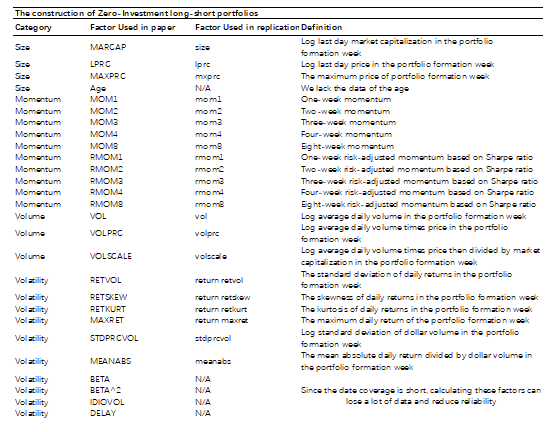
\includegraphics[width=0.7\textwidth]{1.png}
    \caption{Table 1 shows the constructions of different zero-investment long-short.} 
    \label{fig:example}
\end{figure}

portfolios. The main aspects of these 22 factors are size, momentum, volume, and volatility, which we use to form portfolios. Compared to the replicated paper, the age factor was removed due to lack of data. The factors BETA, BETA$^2$, IDIOVOL, and DELAY were also excluded because the date coverage in our model is short, leading to potential data loss and reduced reliability.

We then use these factors to examine stochastic dominance against three asset benchmarks: stock, bond, and risk-free rate.


\hypertarget{replication-of-key-analytical-techniques}{%
\subsection{Replication of Key Analytical
Techniques}\label{replication-of-key-analytical-techniques}}

\subsubsection{Data Preparation}
Prepares the data for calculating returns and the weighted index through loading data1 containing market cap data for top cryptocurrencies and data2 containing trading pairs for top stablecoins and cryptocurrencies. Extract asset information from the market field in data2.

\begin{figure}[h]
    \centering
    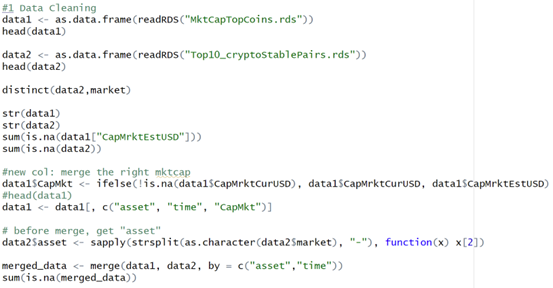
\includegraphics[width=0.7\textwidth]{2.png}
    \label{fig:example}
\end{figure}
Then calculate the Cryptocurrency Log Returns for each cryptocurrency based on its closing price.
\[
\text{log\_daily\_return} = \log\left(\frac{\text{price\_close}}{\text{previous day price\_close}}\right)
\]
Calculate the Market-Capitalization-Weighted Index Return for all the assets on each day (total\_cap), and determines the weight of each asset in the market based on its market cap.
The daily market-cap-weighted index return is computed as the sum of the log daily returns for each cryptocurrency, weighted by their market cap:
\begin{figure}[h]
    \centering
    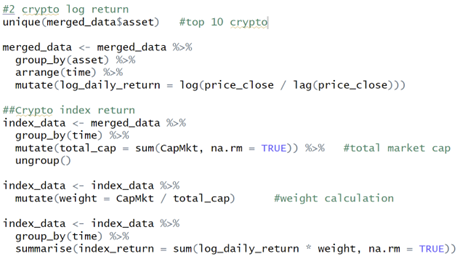
\includegraphics[width=0.7\textwidth]{3.png}
    \label{fig:example}
\end{figure}
\[
\text{index\_return} = \sum (\text{log\_daily\_return} \times \text{weight})
\]
Then we plot the Market-Capitalization-Weighted Index Return and the Market-Capitalization-Weighted Index Value. These plots together provide insights into the daily fluctuations and longer-term trends in the top cryptocurrency market. The index return plot shows the day-to-day variability, while the index value plot demonstrates how the overall market capitalization changes cumulatively over time.

\begin{figure}[h]
    \centering
    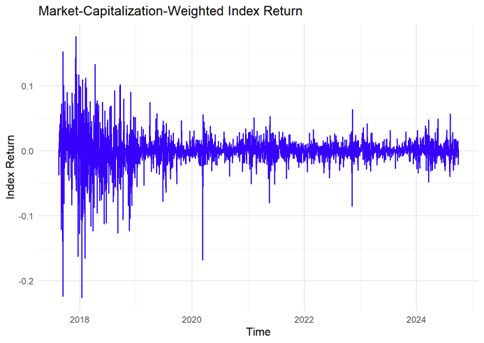
\includegraphics[width=0.7\textwidth]{4.png}
     \caption{The blue line represents the daily returns of a hypothetical index based on the market capitalization of the top 10 cryptocurrencies.}
    \label{fig:example}
\end{figure}
\begin{figure}[h]
    \centering
    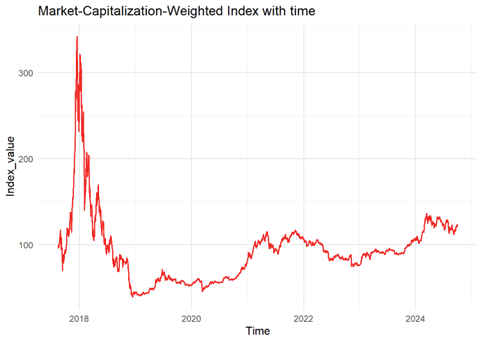
\includegraphics[width=0.7\textwidth]{5.png}
     \caption{The red line shows how the index value evolves over time. It reflects the cumulative effect of the daily returns.}
    \label{fig:example}
\end{figure}

\hypertarget{Set Benchmark: Risk-free and S\&P500}{%
\subsubsection{Set Benchmark: Risk-free and S\&P500}\label{Set Benchmark: Risk-free and S\&P500}}
We combine the benchmark data with the market-capitalization-weighted crypto index return to compare the performance of cryptocurrencies with traditional financial benchmarks of Risk-free and S\&P500.
\begin{figure}[h]
    \centering
    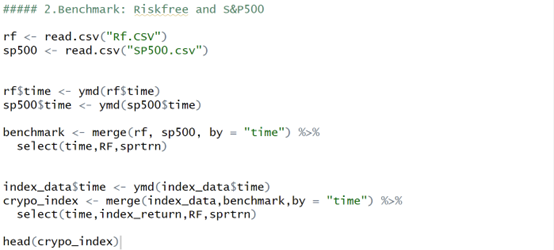
\includegraphics[width=0.7\textwidth]{6.png}
    \label{fig:example}
\end{figure}
\begin{figure}[h]
    \centering
    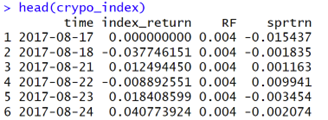
\includegraphics[width=0.7\textwidth]{7.png}
    \label{fig:example}
\end{figure}


\hypertarget{ECDFs Calculating}{%
\subsubsection{ECDFs Calculating}\label{ECDFs Calculating}}

Then calculate the Empirical Cumulative Distribution Functions (ECDFs) for the S\&P 500 returns (sp\_cdf), risk-free rate (rf\_cdf), and the crypto index returns (crypto\_cdf). An ECDF function returns the cumulative probability up to a given value in the input data. For example, for a value x, the ECDF function returns the proportion of data points that are less than or equal to x.
The plot compares the distributions of returns for the crypto index, S\&P 500, and the risk-free rate.
By observing the shape of the CDFs, you can gauge which asset is riskier (steeper increases indicate more concentrated values), which has more variability, and how they perform relative to each other.
\begin{figure}[H]
    \centering
    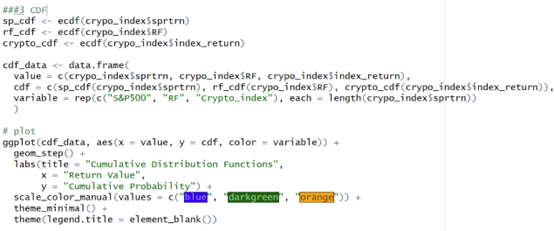
\includegraphics[width=0.7\textwidth]{8.png}
    \label{fig:example}
\end{figure}
\begin{figure}[H]
    \centering
    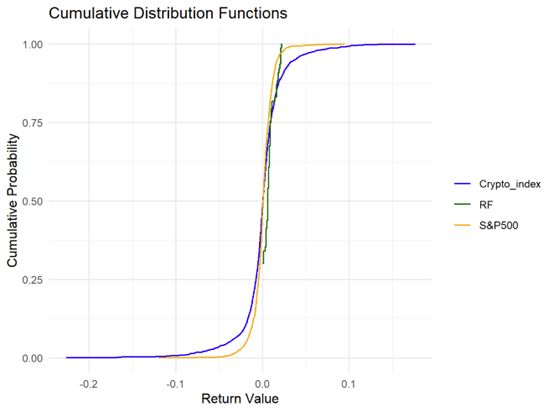
\includegraphics[width=0.7\textwidth]{9.png}
    \label{fig:example}
\end{figure}
\begin{figure}[H]
    \centering
    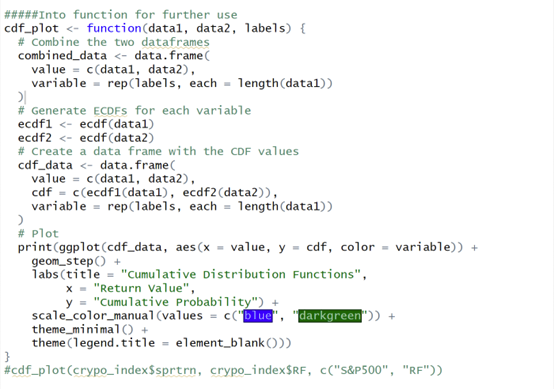
\includegraphics[width=0.7\textwidth]{10.png}
    \label{fig:example}
\end{figure}

Then introduce the cdf\_plot function as a resuable tool for comparing the distribution of two different sets of data. This helps our later modeling of AFSD and ASSD.

\hypertarget{AFSD \& ASSD}{%
\subsubsection{AFSD \& ASSD}\label{AFSD \& ASSD}}
Almost Stochastic Dominance is a concept used in decision theory and finance to compare distributions of returns or outcomes, allowing for some tolerance of violations in the preference ordering. To test whether AFSD and ASSD exist, we need to get the ratio of violation area over the total enclosed area for each portfolio and compare if ratios $\epsilon_1$ (AFSD) and $\epsilon_2$ (ASSD) are lower than AFSD (5.9\%) and ASSD (3.2\%), showing that they meet the requirement.

For AFSD, the FSD violation range is given by:
\[
R_1(F_H, F_L) = \{s \in (r_1, r_2): F_L(s) < F_H(s)\}
\]

The empirical violation area is defined as:
\[
\epsilon_1 = \frac{\int_{R_1} \left[F_H(s) - F_L(s)\right] ds}{\int_{\text{min}}^{\text{max}} \left[F_H(s) - F_L(s)\right] ds}
\]

If $\epsilon_1 < 5.9\%$, AFSD exists.
\begin{figure}[H]
    \centering
    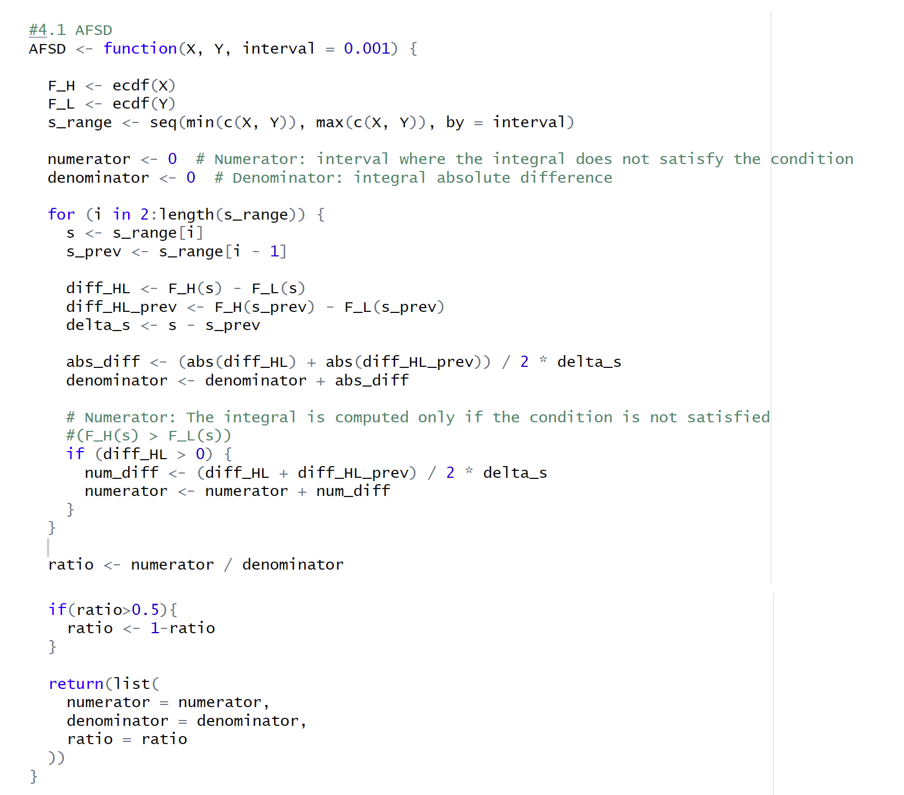
\includegraphics[width=0.7\textwidth]{11.png}
    \label{fig:example}
\end{figure}
For ASSD, the SSD violation range is given by:
\[
R_2(F_H, F_L) = \left\{ s \in (F_H, F_L) : \int_0^r \left[ F_L(s) - F_H(s) \right] ds < 0 \right\}
\]

The empirical violation area is defined as:
\[
\epsilon_2 = \frac{\int_{R_2} \left[ F_H(s) - F_L(s) \right] ds}{\int_{\text{min}}^{\text{max}} \left[ F_H(s) - F_L(s) \right] ds}
\]

If $\epsilon_2 < 3.2\%$, ASSD exists.
\begin{figure}[H]
    \centering
    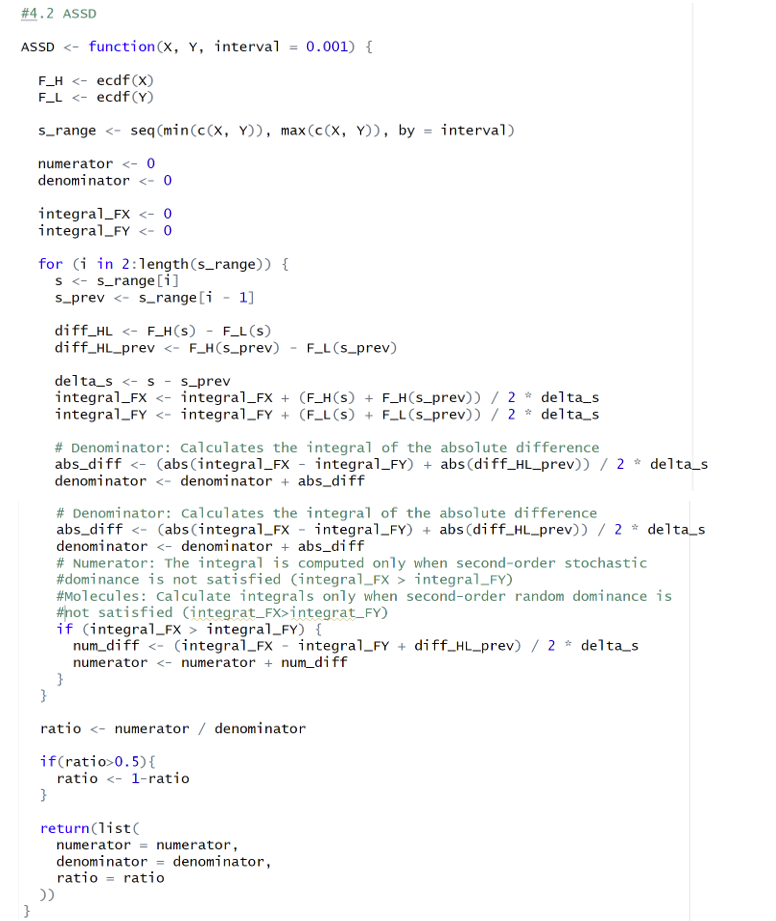
\includegraphics[width=0.7\textwidth]{12.png}
    \label{fig:example}
\end{figure}
\hypertarget{Factor Calculation}{%
\subsubsection{Factor Calculation}\label{Factor Calculation}}


Depend on the previous 22 factors related to the main aspects of size, momentum, volume, and volatility, asset characteristics are calculated.

\paragraph{Momentum Factors:}
Momentum measures the rate of price change over time and is calculated using lagged values of the asset prices.
\begin{itemize}
    \item \textbf{Lagged Values}: Lag1, Lag2, Lag3, Lag4, Lag8 represent the asset's lagged prices over different time periods (7, 14, 21, 28, and 56 days).
    \item \textbf{Momentum (mom)}: Calculated as the difference between the current price and the lagged prices over different time horizons (mom1, mom2, mom3, mom4, mom8). This shows how much the asset's price has changed over those time intervals.
\end{itemize}

\paragraph{Volatility Factors:}
Volatility factors measure the risk and dispersion of returns over various time periods.
\begin{itemize}
    \item \textbf{Standard Deviation (std)}: Calculated over rolling windows of 7, 14, 21, 28, and 56 days (std1, std2, std3, std4, std8). This provides an estimate of how much the price fluctuates within the specified period.
    \item \textbf{Risk-Adjusted Momentum (rmom)}: Momentum is adjusted by dividing by the corresponding standard deviation to account for risk. These are also calculated over different time windows (rmom1, rmom2, rmom3, rmom4, rmom8).
\end{itemize}

\paragraph{Size Factors:}
The size of an asset is generally measured by its market capitalization (\textit{CapMkt}), which is the product of price and the number of shares outstanding.
\begin{itemize}
    \item \textbf{Log-Price (lprc)}: The natural logarithm of the price to stabilize the variance.
    \item \textbf{Max Price (maxprc)}: The maximum price observed over a rolling 7-day window.
\end{itemize}

\paragraph{Volume Factors:}
Volume factors reflect the trading activity and liquidity of the asset.
\begin{itemize}
    \item \textbf{Log-Volume (vol)}: The natural logarithm of the average volume over a rolling 7-day window.
    \item \textbf{Volume-Price Product (volprc)}: The product of volume and price, representing the total traded value.
    \item \textbf{Volume-Scaled Price (volscale)}: Volume-price product divided by market capitalization to assess the liquidity relative to the asset size.
\end{itemize}

The process will compare the portfolios based on ASSD calculations to evaluate if one strategy or factor dominates another.

\paragraph{Quantile:}
Quantile formation involves sorting assets based on factor values and dividing them into equal-sized groups. This method is used to classify assets according to their factor characteristics. For each factor, the assets are divided into five quantiles, and this categorization helps analyze the behavior of portfolios constructed from each quantile.

By categorizing the assets into quantiles for each of these factors, the code enables analysis of portfolio returns, risks, and other metrics. Quantile-based sorting allows for examining if certain factor characteristics (e.g., high momentum or low volatility) result in superior performance.
\begin{figure}[H]
    \centering
    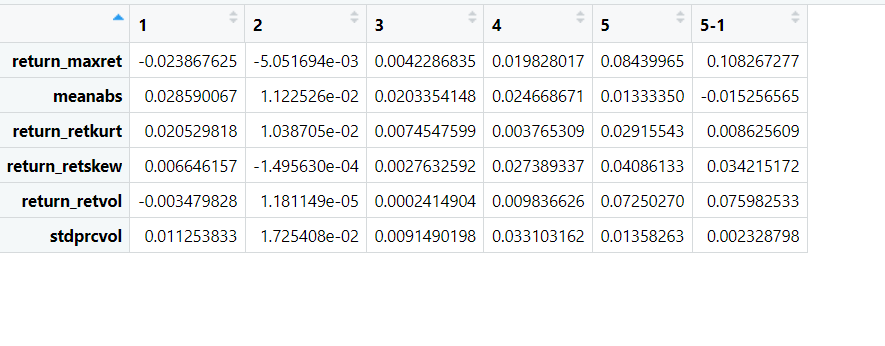
\includegraphics[width=0.7\textwidth]{21.png}
    \label{fig:example}
\end{figure}
\begin{figure}[H]
    \centering
    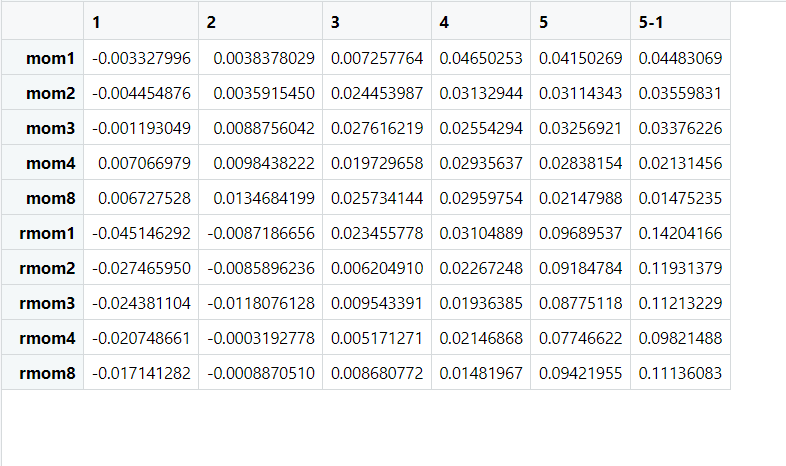
\includegraphics[width=0.7\textwidth]{22.png}
    \label{fig:example}
\end{figure}
\begin{figure}[H]
    \centering
    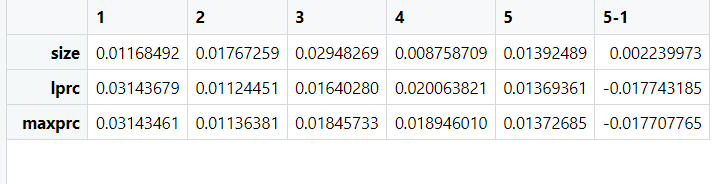
\includegraphics[width=0.7\textwidth]{23.png}
    \label{fig:example}
\end{figure}
\begin{figure}[H]
    \centering
    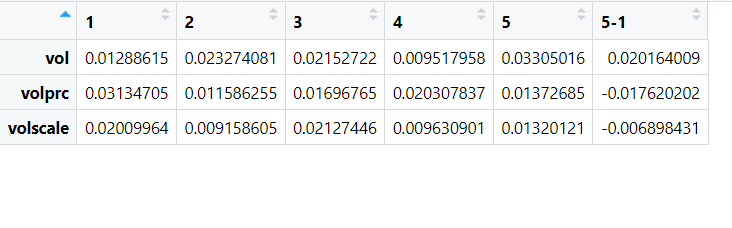
\includegraphics[width=0.7\textwidth]{24.png}
    \label{fig:example}
\end{figure}

\hypertarget{Portfolio Building}{%
\subsubsection{Portfolio Building}\label{Portfolio Building}}
We then analyze financial portfolios, focusing on constructing portfolios based on different factors such as size, momentum, volatility, and volume. Portfolio returns are calculated using equal-weighted and value-weighted methods, with the ultimate goal of assessing the performance of different quantile-based portfolios.

\textbf{Step 1: Portfolio Building}\\
Build various portfolios based on different factors. Combine the size, momentum, volatility, and volume data with the future returns.

\textbf{Step 2: Equal-Weighted Portfolio Calculation}\\
The function \texttt{calculate\_portfolio\_returns()} calculates portfolio returns based on equal weights.

\textbf{The Quantile-Based Long/Short Strategy:}
\begin{itemize}
    \item \textbf{Long Positions}: Assets in the top quantile (5).
    \item \textbf{Short Positions}: Assets in the bottom quantile (1).
    \item The function computes portfolio returns as the difference between the returns from long and short positions.
\end{itemize}

\textbf{Step 3: Value-Weighted Portfolio Calculation}\\
The function \texttt{value\_weighted\_factor\_portfolio()} calculates returns for a value-weighted portfolio as the replicated paper did. The weights of each asset (weights\_port) are calculated by dividing the market value of each asset by the total market value for the period. This normalization ensures that the sum of the weights equals 1. If holding\_period is 1, it uses the default returns (e.g., daily or weekly returns). For longer holding periods, it uses cumulative returns over that period.
This approach ensures that larger assets (by market value) have a more significant impact on the portfolio's returns, following a value-weighted methodology.

\textbf{Step 4: Summary Calculations for Different Factors}\\
Calculates the average returns for different quantiles (1 to 5) across various factors.
\begin{figure}[H]
    \centering
    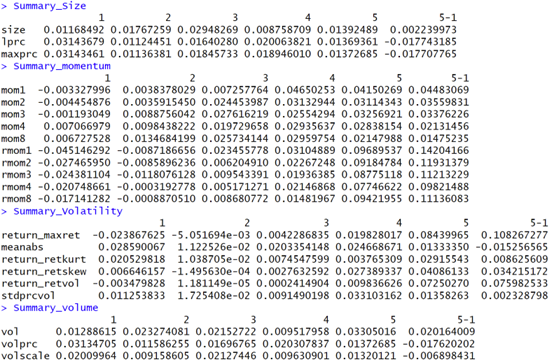
\includegraphics[width=0.7\textwidth]{14.png}
    \label{fig:example}
\end{figure}
\hypertarget{AFSD and ASSD testing and plotting}{%
\subsubsection{AFSD and ASSD testing and plotting}\label{AFSD and ASSD testing and plotting}}

The analysis involves testing AFSD and ASSD across different factors and holding periods, using log returns for the S\&P 500 index as a benchmark.

\textbf{Step 1: Set the Benchmarks of Risk-Free and S\&P 500}\\
Read and prepare weekly log return data for the S\&P 500. This step converts the Date column to a Date format, computes the weekly log returns, and adjusts the dates.
\begin{figure}[H]
    \centering
    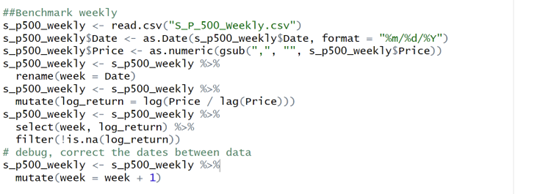
\includegraphics[width=0.7\textwidth]{15.png}
    \label{fig:example}
\end{figure}
\textbf{Step 2: AFSD and ASSD Testing}\\
Compare different factor-based long-short portfolio returns with the S\&P 500 returns. AFSD and ASSD are used to measure the dominance relationships between the long-short portfolio performance and the benchmark.\\
For example, the AFSD and ASSD of size is calculated as follows:
\begin{figure}[H]
    \centering
    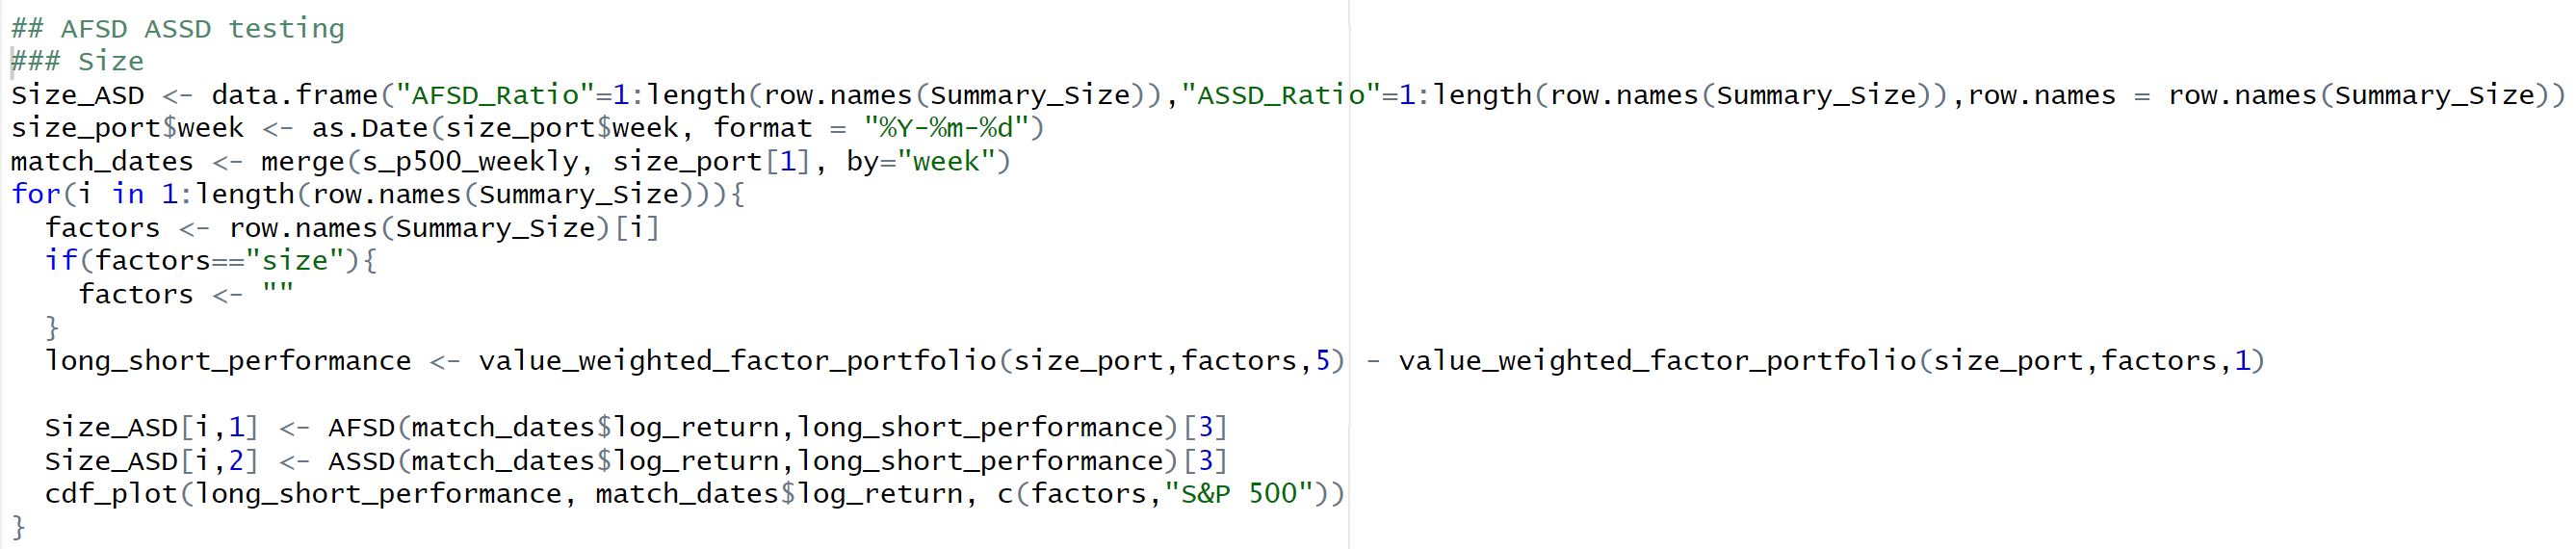
\includegraphics[width=0.7\textwidth]{19.png}
    \label{fig:example}
\end{figure}
Do the same thing for momentum, volatility and volume.\\
\begin{figure}[H]
    \centering
    \begin{subfigure}{0.45\textwidth}
        \centering
        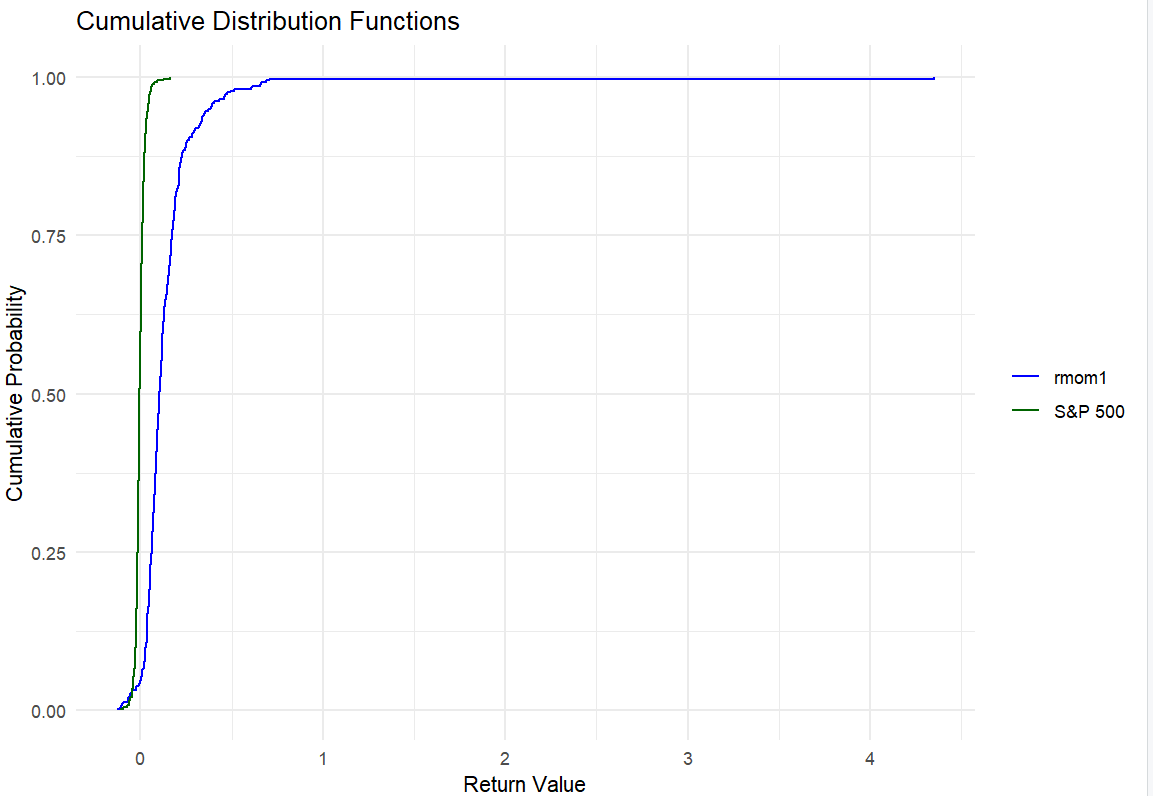
\includegraphics[width=\textwidth]{25.png}
        \label{fig:image25}
    \end{subfigure}
    \hspace{0.05\textwidth}
    \begin{subfigure}{0.45\textwidth}
        \centering
        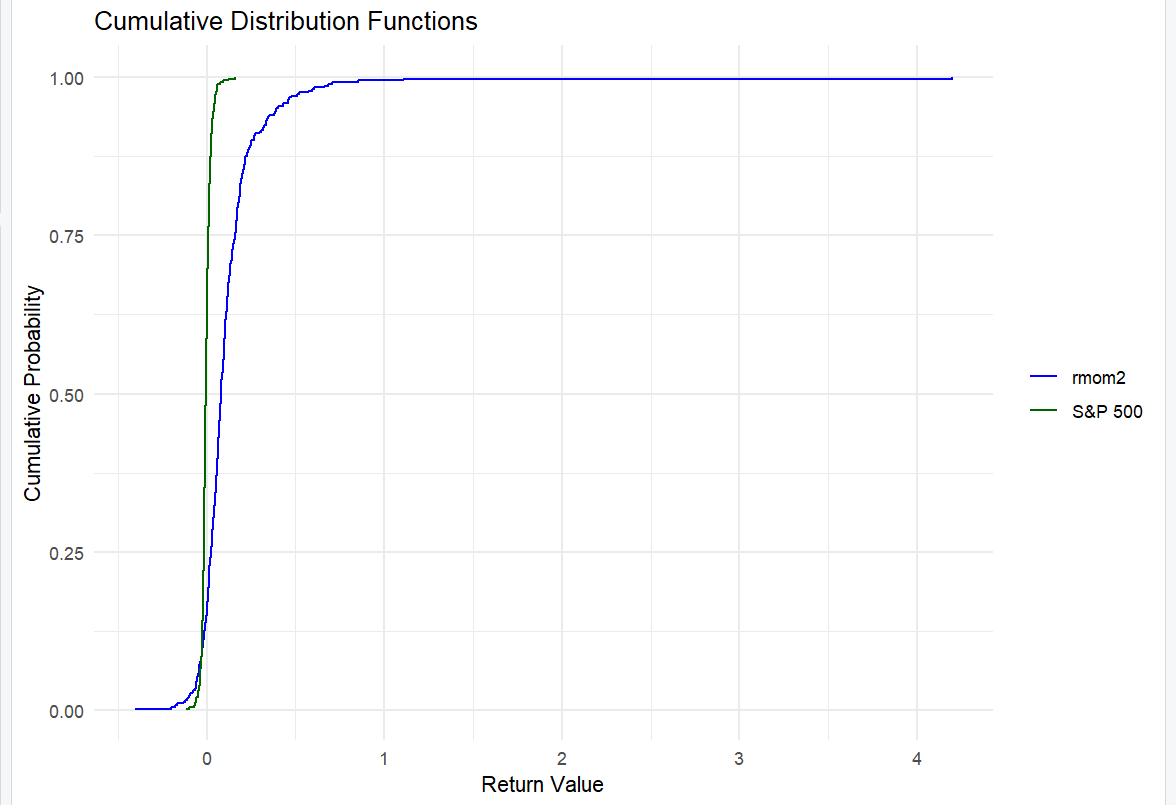
\includegraphics[width=\textwidth]{26.png}
        \label{fig:image26}
    \end{subfigure}

    \begin{subfigure}{0.45\textwidth}
        \centering
        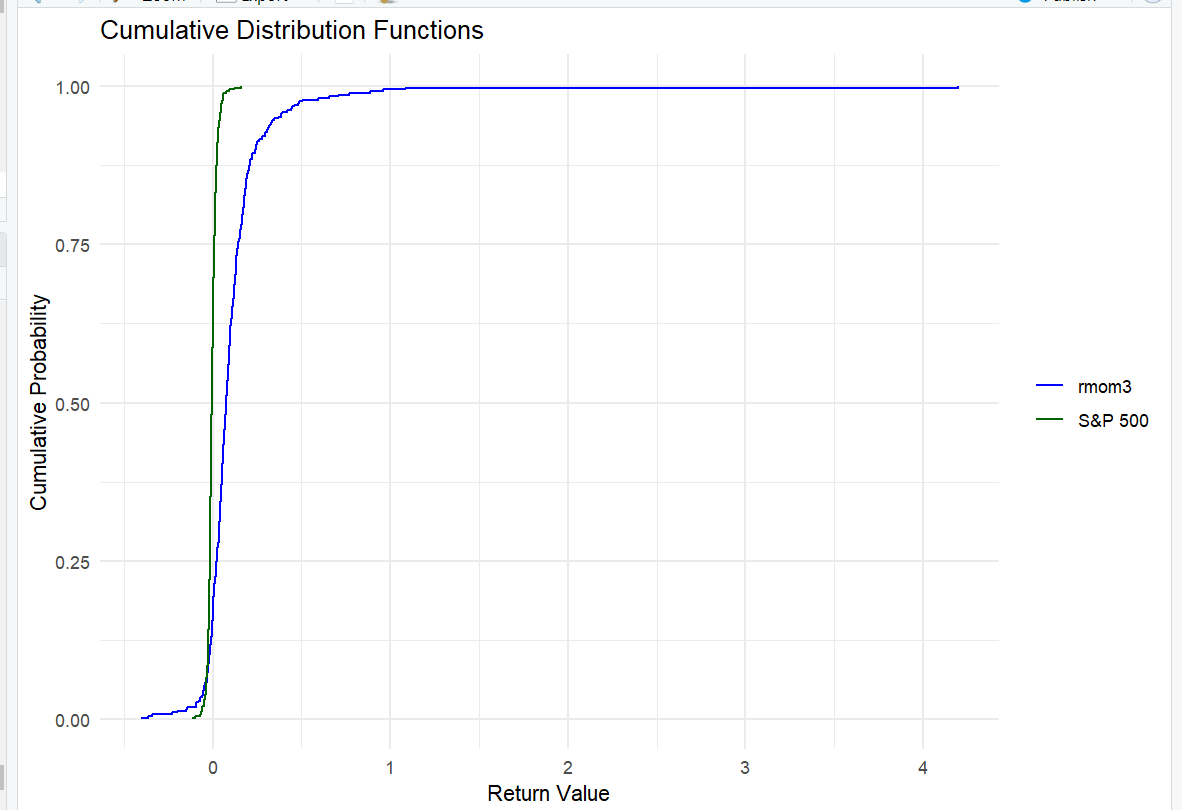
\includegraphics[width=\textwidth]{27.png}
        \label{fig:image27}
    \end{subfigure}
    \hspace{0.05\textwidth}
    \begin{subfigure}{0.45\textwidth}
        \centering
        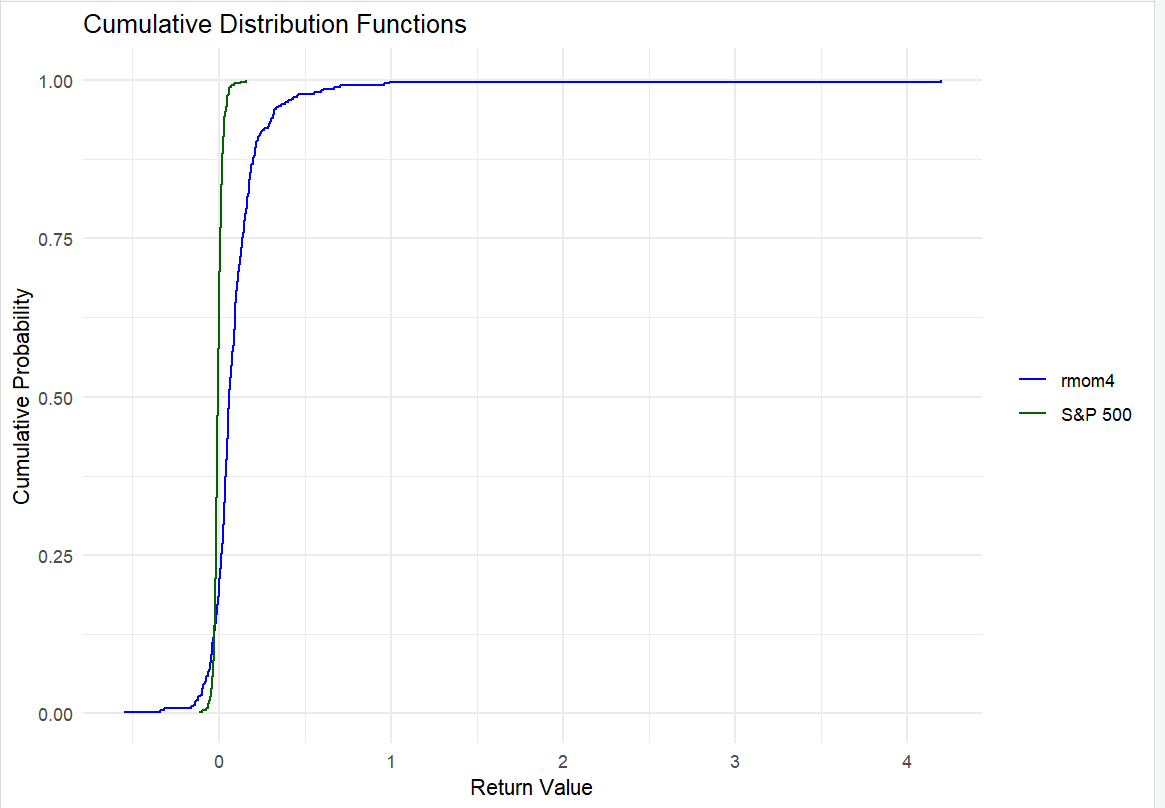
\includegraphics[width=\textwidth]{28.png}
        \label{fig:image28}
    \end{subfigure}
    \label{fig:multiimages}
    \begin{subfigure}{0.45\textwidth}
        \centering
        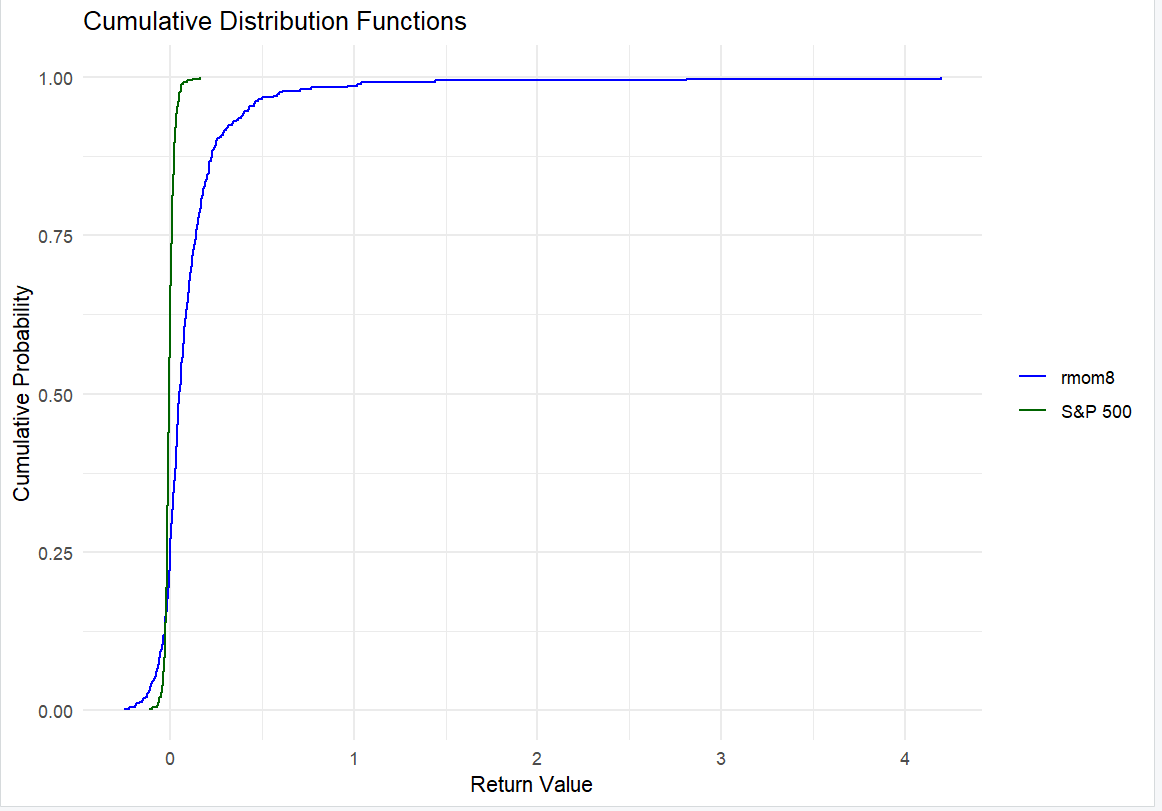
\includegraphics[width=\textwidth]{29.png}
        \label{fig:image29}
    \end{subfigure}
    \hspace{0.05\textwidth}
    \begin{subfigure}{0.45\textwidth}
        \centering
        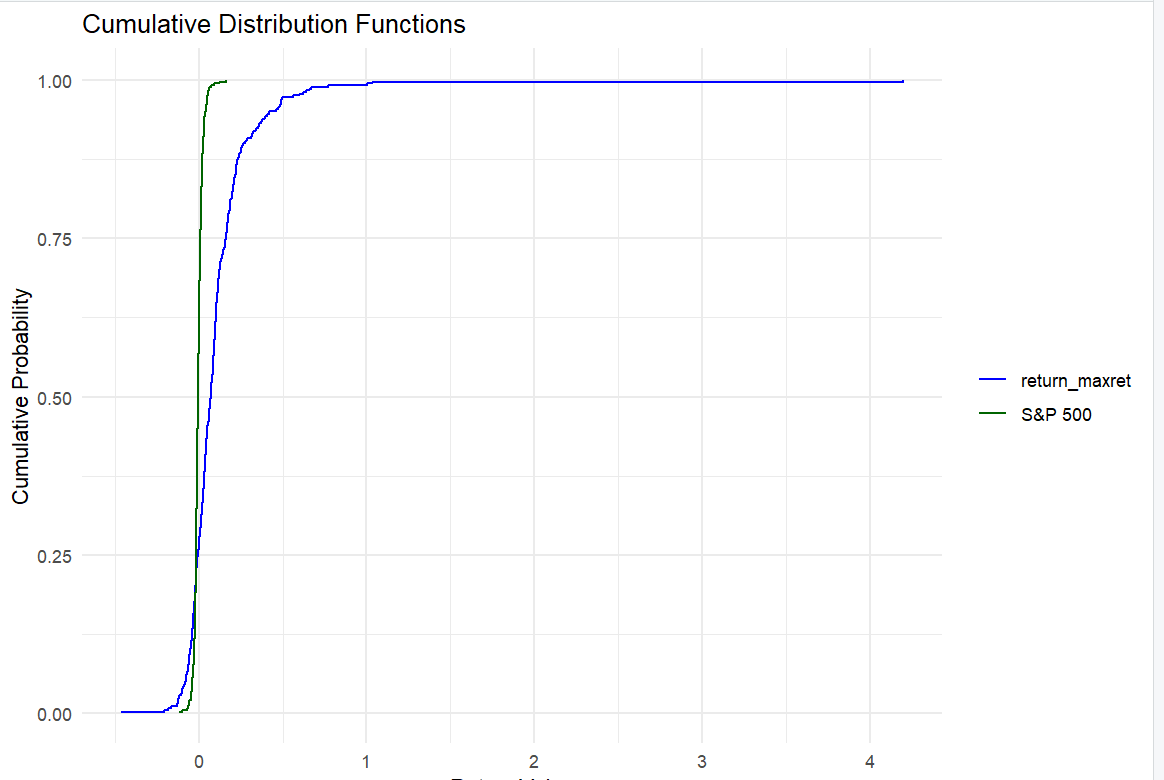
\includegraphics[width=\textwidth]{30.png}
        \label{fig:image30}
    \end{subfigure}

    \begin{subfigure}{0.45\textwidth}
        \centering
        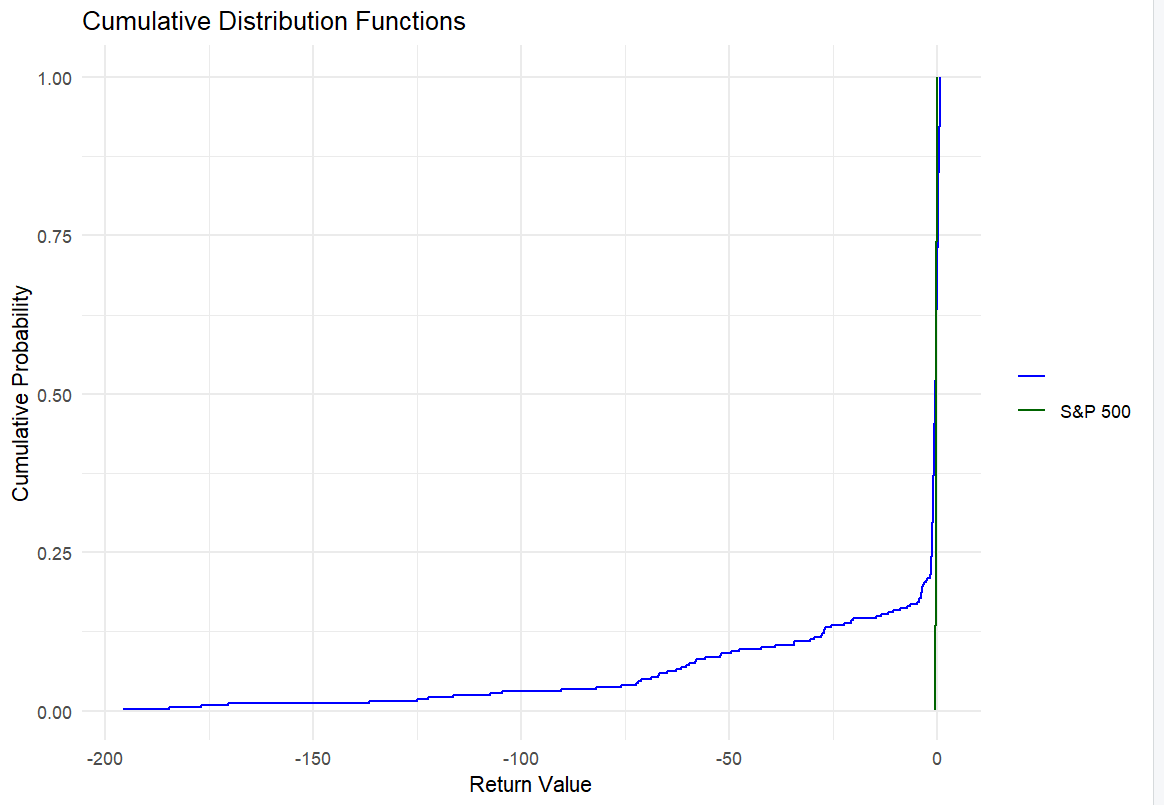
\includegraphics[width=\textwidth]{31.png}
        \label{fig:image31}
    \end{subfigure}
    \hspace{0.05\textwidth}
    \begin{subfigure}{0.45\textwidth}
        \centering
        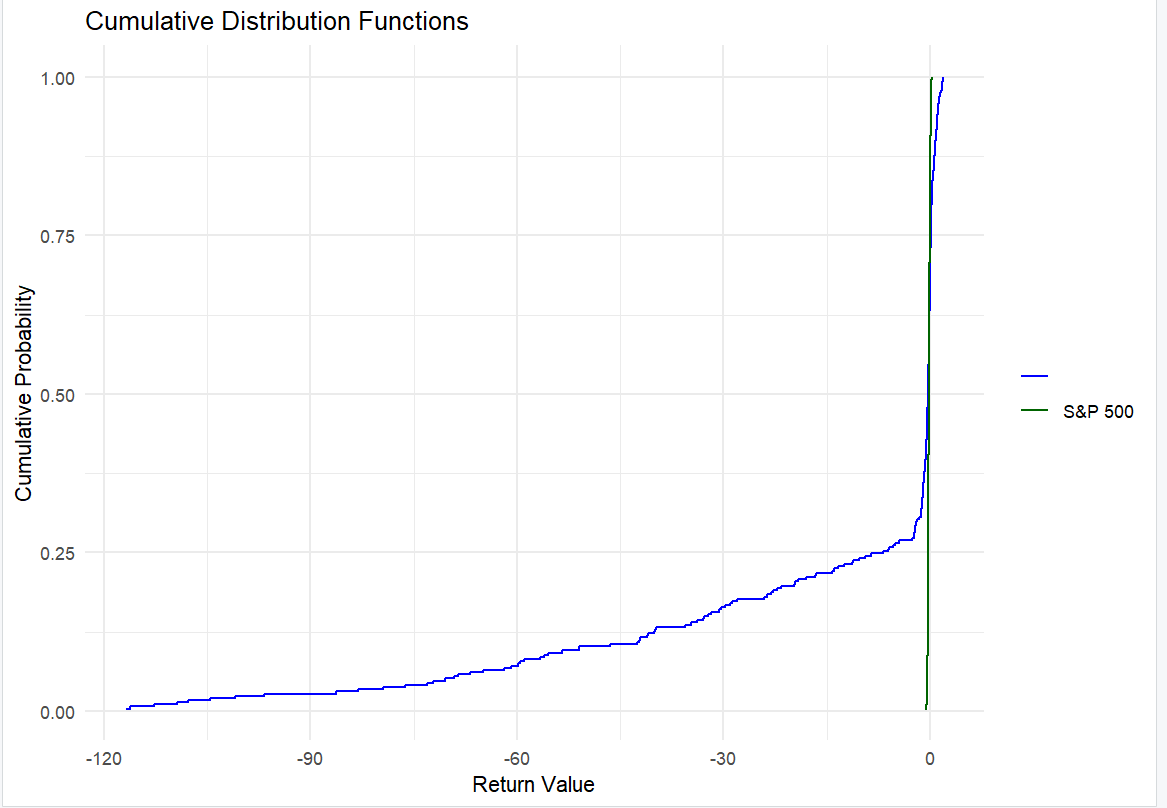
\includegraphics[width=\textwidth]{32.png}
        \label{fig:image32}
    \end{subfigure}
    \label{fig:additional_images}
\end{figure}
\textbf{Step 3: Factor Analysis by Holding Periods}\\
Continue to analyze portfolio performance over different holding periods (4 weeks, 13 weeks, 26 weeks, 52 weeks, and 78 weeks).
For example, apply the different holding periods on momentum as follows:
\begin{figure}[H]
    \centering
    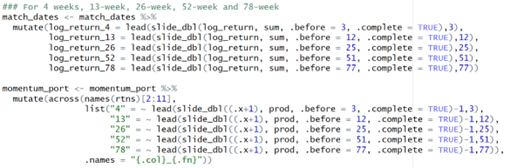
\includegraphics[width=0.5\linewidth]{20.png}
    \label{fig:enter-label}
\end{figure}
Do the same thing for size, volatility and volume.

\textbf{Step 4: Identifying Dominant Factors}\\
Evaluate whether factors exhibit dominance according to AFSD and ASSD criteria. Specific thresholds (5.9\% for AFSD and 3.2\% for ASSD) are used to determine dominance.
\begin{figure}[H]
    \centering
    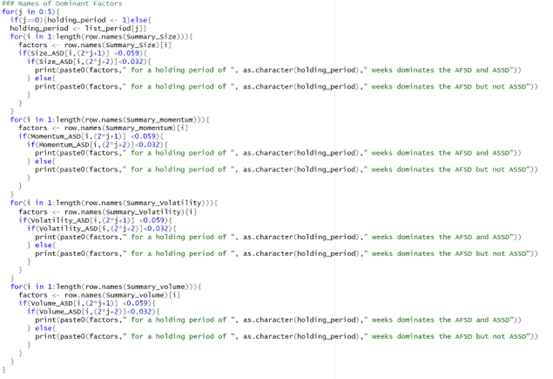
\includegraphics[width=0.7\textwidth]{16.png}
    \label{fig:example}
\end{figure}

\hypertarget{hypothesis-tests}{%
\subsection{Hypothesis Tests}\label{hypothesis-tests}}

After replicating the initial work, it is time to evaluate the hypotheses of the replicated work. We perform hypothesis testing using Almost First-Order Stochastic Dominance (AFSD) and Almost Second-Order Stochastic Dominance (ASSD) to analyze the performance of different investment strategies.

\subsubsection{AFSD and ASSD Testing}

\paragraph{Step 1: Factor-Based Portfolio Construction:}
First, create factor-based long-only and short-only portfolios. For example, portfolios can be constructed based on momentum factors such as rmom1, rmom2, rmom3, rmom4, and rmom8, representing relative momentum over different time periods. The \texttt{value\_weighted\_factor\_portfolio()} function is used to create a long-only portfolio by investing in assets in the top quantile (5) and a short-only portfolio by shorting assets in the bottom quantile (1).
\begin{figure}[H]
    \centering
    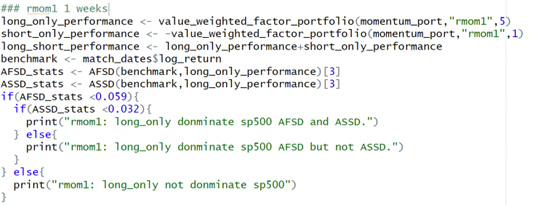
\includegraphics[width=0.7\textwidth]{17.png}
    \label{fig:example}
\end{figure}
\paragraph{Step 2: Long-Short Portfolio Creation:}
The long-short portfolio is calculated by adding the returns of the long-only portfolio and the negative returns of the short-only portfolio.

\paragraph{Step 3: Benchmark Data Preparation:}
The benchmark data used for comparison is the log returns of the S\&P 500 index, stored in the benchmark variable.

\paragraph{Step 4: AFSD and ASSD Testing:}
The \texttt{AFSD()} and \texttt{ASSD()} functions calculate the Almost Stochastic Dominance statistics for various combinations of portfolios and the benchmark. Specifically, the tests are conducted to determine whether:
\begin{itemize}
    \item The long-only portfolio dominates the benchmark.
    \item The short-only portfolio dominates the benchmark.
    \item The short-only portfolio dominates the long-only portfolio.
    \item The short-only portfolio dominates the long-short portfolio.
    \item The long-short portfolio dominates the long-only portfolio.
\end{itemize}

\paragraph{Step 5: Decision Criteria for Stochastic Dominance}
If the AFSD statistic is less than 0.059, it indicates that the tested portfolio might dominate the comparison portfolio based on AFSD. If the ASSD statistic is less than 0.032, it indicates dominance based on ASSD. Based on these thresholds, the code prints statements about the dominance relationships between portfolios.
\begin{figure}[H]
    \centering
    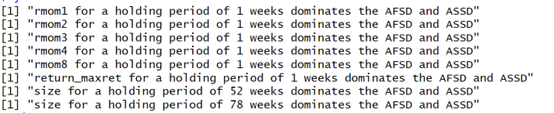
\includegraphics[width=0.7\textwidth]{18.png}
    \label{fig:example}
\end{figure}
\paragraph{Analysis of the Results}
\begin{itemize}
    \item \textbf{Short-Term Dominance (1 Week):} The momentum factors rmom1, rmom2, rmom3, rmom4, and rmom8 dominate both AFSD and ASSD for a 1-week holding period. This suggests that momentum strategies are highly effective in generating superior returns over short-term horizons. The volatility factor return\_maxret also dominates AFSD and ASSD in the 1-week holding period, indicating that maximum return volatility strategies outperform the S\&P 500 in the very short term.
    \item \textbf{Long-Term Dominance (52 and 78 Weeks):} The size factor dominates both AFSD and ASSD for holding periods of 52 weeks and 78 weeks, suggesting that size-based investment strategies yield better long-term performance compared to the benchmark.
\end{itemize}

\paragraph{Step 6: Testing Across Different Factors}
The code repeats the process for various momentum factors (rmom1 to rmom8) and size-based portfolios (size\_52\_weeks and size\_78\_weeks), considering different holding periods (52 weeks and 78 weeks).

\subsubsection{Hypothesis 2 Testing}
Since the above factors all dominate the AFSD and ASSD, further testing is used to form strategies that evaluate the performance of different trading strategies using AFSD and ASSD criteria. The strategies tested include long-only, short-only, and long-short portfolios, which are compared to the benchmark (S\&P 500) and to each other.

\paragraph{Calculate Performances}
\begin{itemize}
    \item \textbf{long\_only\_performance}: The performance of a long-only strategy, which involves buying assets in the highest quantile (top 20\%) for the factor rmom1.
    \item \textbf{short\_only\_performance}: The performance of a short-only strategy, which involves shorting assets in the lowest quantile (bottom 20\%) for the factor rmom1.
    \item \textbf{long\_short\_performance}: The combination of both strategies, calculated as the sum of long-only and short-only performances.
\end{itemize}

\paragraph{AFSD and ASSD Tests}
For example, for rmom1:
\begin{itemize}
    \item \textbf{rmom1: Long-Only vs. S\&P 500}: The long-only strategy does not dominate the benchmark for both AFSD and ASSD, indicating that it does not outperform the S\&P 500 based on the stochastic dominance criteria.
    \item \textbf{rmom1: Short-Only vs. S\&P 500}: The short-only strategy also fails to dominate the benchmark.
    \item \textbf{rmom1: Short-Only vs. Long-Only}: The short-only strategy dominates the long-only strategy for both AFSD and ASSD criteria. This suggests that shorting assets in the lowest quantile performs better than buying assets in the highest quantile for this factor over the 1-week period.
    \item \textbf{rmom1: Short-Only vs. Long-Short}: The short-only strategy also outperforms the combined long-short strategy based on both stochastic dominance criteria.
    \item \textbf{rmom1: Long-Short vs. Long-Only}: The combined long-short strategy dominates the long-only strategy, suggesting that a mixed approach of both buying high-quantile assets and shorting low-quantile assets yields better performance than a pure long strategy.
\end{itemize}

Do the same thing for the rest of the factors. The hypothesis is tested across various factors, including different momentum measures (rmom1, rmom3, rmom4, rmom8) and a size factor over longer holding periods (52 and 78 weeks).

\subsubsection{Results}
\begin{itemize}
    \item \textbf{Momentum Factors (rmom1, rmom3, rmom4, rmom8):}
    \begin{itemize}
        \item \textbf{Long-Only vs. S\&P 500}: For all momentum factors tested, the long-only strategy does not dominate the S\&P 500 for both AFSD and ASSD, indicating that a long-only approach may not outperform the benchmark.
        \item \textbf{Short-Only vs. S\&P 500}: Similarly, the short-only strategy fails to dominate the S\&P 500, suggesting it does not provide better returns than the benchmark.
        \item \textbf{Short-Only vs. Long-Only}: In each case, the short-only strategy dominates the long-only strategy for both AFSD and ASSD criteria, suggesting that shorting low-ranked assets yields better performance than buying high-ranked assets in the momentum context.
        \item \textbf{Short-Only vs. Long-Short}: The short-only strategy also dominates the long-short strategy across all momentum factors, indicating that pure shorting is more effective than combining long and short positions.
        \item \textbf{Long-Short vs. Long-Only}: In some cases (like rmom1), the long-short strategy dominates the long-only strategy, suggesting that including short positions improves performance over a pure long strategy.
    \end{itemize}
    \item \textbf{Size Factor for Longer Holding Periods:}
    \begin{itemize}
        \item \textbf{52 Weeks}: The long-only strategy dominates the S\&P 500 in both AFSD and ASSD for a 52-week holding period, indicating strong performance.
        \item \textbf{Short-Only vs. S\&P 500}: The results for short-only dominance were not provided, but it can be inferred that it would not outperform the S\&P 500 based on previous patterns.
    \end{itemize}
\end{itemize}

These results highlight the importance of strategy selection and factor timing in portfolio management, where momentum shorting may be effective in the short term, while size factors offer potential over longer horizons.

\hypertarget{future-work}{%
\section{Future Work}\label{future-work}}

Future research could extend the analysis by examining longer investment horizons and incorporating different asset classes, such as commodities or real estate, to better understand the performance of cryptocurrency factors over time and across a broader investment landscape. Additionally, investigating the impact of various market conditions (e.g., bull vs. bear markets) on factor dominance could provide insights into the conditional performance of cryptocurrency investments.

\hypertarget{conclusions}{%
\section{Conclusions}\label{conclusions}}

This analysis utilizes non-parametric almost stochastic dominance (AFSD and ASSD) to evaluate the performance of various portfolio strategies based on different factors, including momentum and size, to determine if they can outperform a benchmark of the S\&P 500 over different time horizons (1 to 78 weeks). Our findings reveal dominant factors in the short term (1-week) for momentum-based strategies (rmom1, rmom3, rmom4, and rmom8), where short-only portfolios consistently dominate long-only portfolios in terms of both AFSD and ASSD criteria. This suggests that shorting low-ranked assets is more effective than buying high-ranked assets in momentum strategies. Additionally, we find that long-short strategies generally perform better than long-only strategies, particularly for short-term momentum factors.

In the longer term (52 and 78 weeks), the size factor exhibits significant dominance over the benchmark, with long-only portfolios outperforming the S\&P 500 under both AFSD and ASSD. This indicates that size-based strategies may be more effective over extended horizons. However, for shorter momentum strategies, long-only approaches do not dominate the benchmark, highlighting limitations in using such strategies in isolation.

Our analysis supports the value of incorporating short positions in portfolio management, particularly for momentum strategies, and suggests that size factors can be effective for long-term investment horizons. However, further research is warranted to explore the performance of additional factors, the impact of different market conditions, and alternative risk metrics to enhance understanding of these strategies.


\newpage

\begin{figure}
\centering

\includegraphics{cc_by_88x31.png}
\caption{CC-BY}
\end{figure}

\hypertarget{references}{%
\section*{References}\label{references}}



\end{document}
